\section{Basics of linear problems}


%TODO: Chp2: It would be more natural to start with the convexity of polyhedral sets and then move on to the linear algebra definitions. We just need to be careful to define the elements needed (halfspaces, hyperplanes, etc) so the presentation of convexity elements make sense 

As we have seen in the previous chapter, the feasible region of a linear programming problem can be represented as
%
\begin{equation} \label{p1c2:eq:feasible_region_inequality}
	Ax \leq b,	
\end{equation}

where $A$ is a $m \times n$ matrix, $x$ is a $n$-dimensional column vector (or more compactly, $x \in \reals^n$), and $b$ is an $m$-dimensional column vector ($b \in \reals^m$). Notice that $\leq$ is considered component-wise. Also, let $\dim(x)$ denote the dimension of vector $x$.

Before introducing the simplex method, let us first revisit a few key elements and operations that we will use in the process. The first of them is presented in Definition \ref{p1c2:def:matrix_inversion}.
%
\begin{definition}[Matrix inversion] \label{p1c2:def:matrix_inversion}
	Let $A$ be a square $n \times n$ matrix. $A^{-1}$ is the inverse matrix of $A$ if it exists and $AA^{-1} = I$, where  $I$ is the ($n \times n$) identity matrix.
\end{definition}
%
Matrix inversion is the ``kingpin'' of linear (and nonlinear) optimisation. As we will see later on, performing efficient matrix inversion operations (in reality, operations that are equivalent to matrix inversion but that can exploit the matrix structure to be made faster) is of utmost importance for developing a linear optimisation solver. 

Another important concept is the notion of \emph{linear independence}. We formally state when a collection of vectors is said to be linearly independent (or dependent) in Definition \ref{p1c2:def:linear_independence}. 

%
\begin{definition}[Linearly independent vectors] \label{p1c2:def:linear_independence}
	The vectors $\braces{x_i}_{i=1}^k \in \reals^n$  are linearly dependent if there exist real numbers $\braces{a_i}_{i=1}^k$ with $a_i \neq 0$ for at least one $i \in \braces{1,\dots, k}$ such that
	$$
		\sum_{i=1}^k a_i x_i= 0;
	$$
	otherwise, $\braces{x_i}_{i=1}^k$ are linearly independent.
\end{definition}

In essence, for a collection of vectors to be linearly independent, it must be so that none of the vectors in the collection can be expressed as a linear combination (that is, multiplying the vectors by nonzero scalars and adding them) of the others. Analogously, they are said to be linearly dependent if one vector in the collection can be expressed as a linear combination of the others. 

This is simpler to see in $\reals^2$. Two vectors are linearly independent if one cannot obtain one by multiplying the other by a constant, which effectively means that they are not parallel. If the two vectors are not parallel, then one of them must have a component in a direction that the other vector cannot ``reach''. The same idea can be generalised to any $n$-dimensional space. Also, that explains why one can only have up to $n$ independent vectors in $\reals^n$. Figure \ref{p1c2:fig:linear_independence} illustrates this idea. 

\begin{figure}[h]
	\centering
    \begin{tikzpicture}
%	    \draw[help lines] (-2,-2) grid (2,3);
		\node (pic) at (0,0) {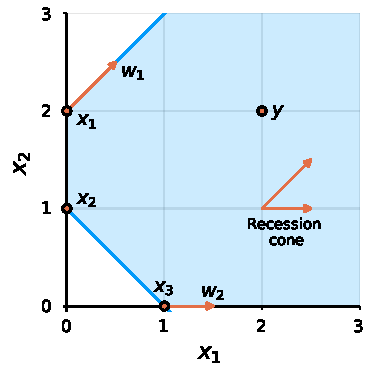
\includegraphics{part_1/chapter_2/figures/Figure1}};
		\node (x1) at (-1.7, 2.1) {$x_1$};
		\node (x2) at (1.2, 2.2) {$x_2$};
		\node (x11) at (-1.9, -0.2) {$x_1$};
		\node (x12) at (1, 0) {$x_2$};
		\node (x3) at (2.1, -0.8) {$x_3$};
    \end{tikzpicture}
	\caption{Linearly independent (top) and dependent (bottom) vectors in $\reals^2$. Notice how, in the bottom picture, any of the vectors can be obtained by appropriately scaling and adding the other two}\label{p1c2:fig:linear_independence}
\end{figure}

Theorem \ref{p1c2:thm:fundamental_linear_algebra} summarises results that we will utilise in the upcoming developments. These are classical results from linear algebra and the proof is left as an exercise.
%
\begin{theorem}[Inverses, linear independence, and solving $Ax = b$] \label{p1c2:thm:fundamental_linear_algebra}
	Let $A$ be a $m \times m$ matrix. Then, the following statements are equivalent:
	\begin{enumerate}
		\item $A$ is invertible
		\item $A^\top$ is invertible
		\item The determinant of $A$ is nonzero
		\item The rows of $A$ are linearly independent
		\item The columns of $A$ are linearly independent
		\item For every $b \in \reals^m$, the linear system $Ax = b$ has a unique solution
		\item There exists some $b \in \reals^m$ such that $Ax = b$ has a unique solution.	
	\end{enumerate}	
\end{theorem}
%
Notice that Theorem \ref{p1c2:thm:fundamental_linear_algebra} establishes important relationships between the geometry of the matrix $A$ (its rows and columns) and consequences it has to our ability to calculate its inverse $A^{-1}$ and, consequently, solve the system $Ax = b$, to which the solution is obtained as $x = A^{-1}b$. Solving linear systems of equations will turn out to be the most important operation in the simplex method.


\subsection{Subspaces and bases}

Let us define some objects that we will frequently refer to. The first of them is the notion of a \emph{subspace}. A subspace of $\reals^n$ is a set comprising all linear combinations of its own elements. Specifically, if $S$ is a subspace, then
%
\begin{equation*}
	S = \braces{ax + by : x,y \in S; a,b \in \reals}.
\end{equation*}
%
A related concept is the notion of a \emph{span}. A span of a collection of vectors $\braces{x_i}_{i=1}^k \in \reals^n$ is the subspace of $\reals^n$ formed by all linear combinations of such vectors, i.e., 
%
\begin{equation*}
	\spans(x_1,\dots, x_k) = \braces{y = \sum_{i=1}^k a_ix_i : a_i \in \reals, i \in \braces{1,\dots, k}}. 
\end{equation*}
%
Notice how the two concepts are related: the span of a collection of vectors forms a subspace. Therefore, a subspace can be characterised by the collection of vectors whose span forms it. In other words, the span of a set of vectors is the subspace formed by all points we can represent by some linear combination of these vectors. 

The missing part in this is the notion of a \emph{basis}. A \emph{basis} of the subspace $S \subseteq \reals^n$ is a collection of vectors $\braces{x_i}_{i=1}^k \in \reals^n$ that are linearly independent such that $\spans(x_1,\dots, x_k) = S$. 

Notice that a basis is a ``minimal'' set of vectors that form a subspace. You can think of it in light of the definition of linearly independent vectors (Definition \ref{p1c2:def:linear_independence}); if a vector is linearly dependent to the others, it is not needed for characterising the subspace that the vectors span since it can be represented by a linear combination of the other vectors (and thus is in the subspace formed by the span of the other vectors).

The above leads us to some important realisations:

\begin{enumerate}
	\item All bases of a given subspace $S$ have the same dimension. Any extra vector would be linearly dependent to those vectors that span $S$. In that case, we say that the subspace has size (or dimension) $k$, the number of linearly independent vectors forming the basis of the subspace. We can overload the notation $\dim(S)$ to represent the dimension of the subspace $S$.
	\item If the subspace $S \subset \reals^n$ is formed by a basis of size $m < n$, we say that $S$ is a proper subspace with $\dim(S)=m$, because it is not the whole $\reals^n$ itself, but a space contained within $\reals^n$. For example, two linearly independent vectors form (i.e., span) a hyperplane in $\reals^3$; this hyperplane is a proper subspace since $\dim(S)=m=2 < 3=n$.
	\item If a proper subspace has dimension $m < n$, then it means that there are $n-m$ directions in $\reals^n$ that are perpendicular to the subspace and to each other. That is, there are nonzero vectors $a_i$ that are orthogonal to each other and to $S$. Or, equivalently, $a_i^\top x = 0$ for $i = n-m + 1, ..., n$. Referring to the $\reals^3$, if $m=2$, then there is a third direction that is perpendicular to (or not in) $S$. Figure \ref{p1c2:fig:proper_subpaces} can be used to illustrate this idea. Notice how one can find a vector, say $x_3$ that is perpendicular to $S$. This is because the whole space is $\reals^3$, but $S$ has dimension $m=2$ (or $\dim(S)=2$). 
\end{enumerate}

\begin{figure}
	\centering
	\begin{tikzpicture}
%			\draw[help lines] (-4,-2) grid (4,2);
		\node (pic) at (0,0) {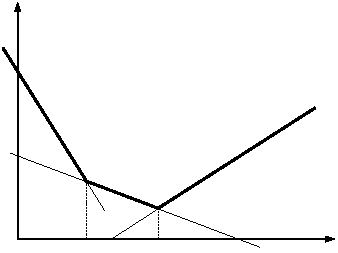
\includegraphics{part_1/chapter_2/figures/Figure2}};
		\node (x1l) at (-1.6, 0.6) {$x_1$};
		\node (Sl) at (-1.1, 0.9) {$S$};	
		\node (x1r) at (2.8, 0.8) {$x_1$};
		\node (x2r) at (2.6, -0.9) {$x_2$};
		\node (Sr) at (3.7, -0.3) {$S$};
	\end{tikzpicture}
	\vspace{-12pt}
	\caption{One- (left) and two-dimensional subspaces (right) in $\reals^3$.} \label{p1c2:fig:proper_subpaces}
\end{figure}

Theorem \ref{p1c2:thm:LI_and_bases} builds upon the previous points to guarantee the existence of bases and propose a procedure to form them.

\begin{theorem}[Forming bases from linearly independent vectors]\label{p1c2:thm:LI_and_bases}
	Suppose that $S = \spans(x_1,\dots, x_k)$ has dimension $m \leq k$. Then
	\begin{enumerate}
		\item There exists a basis of $S$ consisting of $m$ of the vectors $x_1,\dots, x_k$.
		\item If $k' \leq m$ and $x_1,\dots, x_{k'} \in S$ are linearly independent, we can form a basis for $S$ by starting with $x_1,\dots, x_{k'}$ and choosing $m-{k'}$ additional vectors from $x_1,\dots, x_k$.
	\end{enumerate}	
\end{theorem}

\begin{proof}
	Notice that, if every vector $x_{k'+1}, \dots, x_{k}$ can be expressed as a linear combination of $x_{1},\dots x_{k'}$, then every vector in $S$ is also a linear combination of $x_{1}, \dots, x_{k'}$. Thus, $x_{1}, \dots, x_{k'}$ form a basis to $S$ with $m =k'$. Otherwise, at least one of the vectors in $x_{k'+1}, \dots, x_{k}$ is linearly independent from $x_{1}, \dots, x_{k'}$. By picking one such vector, we now have $k'+1$ of the vectors $x_{k'+1}, \dots, x_{k}$ that are linearly independent. If we repeat this process $m - k'$ times, we end up with a basis for $S$.
\end{proof}


Our interest in subspaces and bases spans (pun intended!) from their usefulness in explaining how the simplex method works under a purely algebraic (as opposed to geometric) perspective. For now, we can use the opportunity to define some ``famous'' subspaces which will often appear in our derivations. 

Let $A$ be a $m \times n$ matrix. The \emph{column space} of $A$ consists of the subspace spanned by the $n$ columns of $A$ and has dimension $m$ (recall that each column has as many components as the number of rows and is thus a $m$-dimensional vector). Likewise, the \emph{row space} of $A$ is the subspace in $\reals^n$ spanned by the rows of $A$. Finally, the \emph{null space} of $A$, often denoted as $\nulls(A) = \braces{x \in \reals^n : Ax = 0}$, consist of the vectors that are perpendicular to the row space of $A$. 

One important notion related to those subspaces is their size. Both the row and the column space have the same size, which is the \emph{rank} of $A$. If $A$ is \emph{full rank}, than it means that 
%
\begin{equation*}
	\rank(A) = \min \braces{m,n}. 		
\end{equation*}
%
Finally, the size of the null space of $A$ is given $n - \rank(A)$, which is in line with Theorem \ref{p1c2:thm:LI_and_bases}.


\subsection{Affine subspaces}

A related concept is that of an \emph{affine subspace}. Differently from linear subspaces (to which we have been referring to simply as subspaces), affine subspaces encode some form of translation, such as  
%
\begin{equation*}
	S = S_0 + x_0 = \braces{x + x_0 : x \in S_0}.
\end{equation*}
%
Affine subspaces differ from linear subspaces because they do not contain the origin (recall that the definition of subspaces allows for $a$ and $b$ to be zero). Nevertheless, $S$ has the \emph{same dimension} as $S_0$.

Affine subspaces give a framework for representing linear programming problems algebraically. Specifically, let $A$ be a $m \times n$ matrix with $m < n$ and $b$ a $m$-dimensional vector. Then, let 
%
\begin{equation} \label{p1c2:eq:equality_constraint_feasible_set}
	S = \braces{x \in \reals^n : Ax = b}.		
\end{equation}
%
As we will see, the feasible set of any linear programming problem can be represented as an equality-constrained equivalent of the form of \eqref{p1c2:eq:equality_constraint_feasible_set} by adding slack variables to the inequality constraints, meaning that we will always have that $m < n$.  Now, assume that $x_0 \in \reals^n$ is such that $Ax_0 = b$.  Then, we have that 
%
\begin{equation*}
	Ax = Ax_0 = b \Rightarrow A(x - x_0) = 0.	
\end{equation*}
%
Thus, $x \in S$ if and only if the vector $(x - x_0)$ belongs to $\nulls(A)$, the nullspace of $A$. Notice that the feasible region $S$ can be also defined as 
%
\begin{equation*}
	S = \braces{x + x_0 : x \in \nulls(A)},	
\end{equation*}
%
being thus an affine subspace with dimension $n-m$, if $A$ has $m$ linearly independent rows (i.e., $\rank(A)=m$). This will have important implications in the way we can define multiple bases for $S$ from the $n$ vectors in the column space and what implications it has for the feasibility of the whole problem. Figure \ref{p1c2:fig:nill_space_a} illustrates this concept for a single-row matrix $a$. For a multiple-row matrix $A$, $S$ becomes the intersection of multiple hyperplanes.

\begin{figure}
	\begin{tikzpicture}
	    \node (pic) at (0,0) {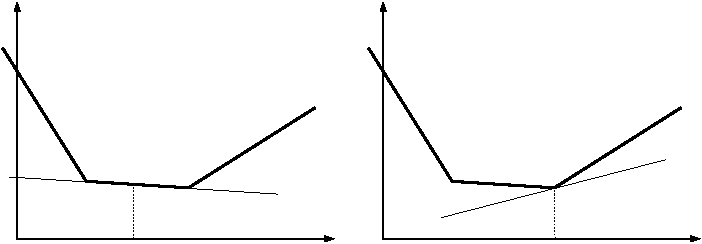
\includegraphics{part_1/chapter_2/figures/Figure3}};
	    \node (x0) at (0,-0.4) {$x_0$};
	    \node (x1) at (1.4,0.4) {$x_1$};
	    \node (x2) at (-1,-0.9) {$x_2$};
	    \node (a) at (-0.5,1.4) {$a$};
	    \node (S) at (-1.7,0.2) {$S$}; 
	\end{tikzpicture}
	\caption{The affine subspace $S$ generated by $x_0$ and $\nulls(a)$. Notice that all vectors in $S$, exemplified by $x_1$ and $x_2$ are perpendicular (i.e., have null dot product) to $a$} \label{p1c2:fig:nill_space_a}.		
\end{figure}


\section{Convex polyhedral set}

The feasible region of any linear programming problem is a convex polyhedral set, which we will simply refer to as a polyhedral set. That is because we are interested in polyhedral sets that are formed by an intersection of a finite number of half-spaces and can thus only be convex (as we will see in a moment), creating redundancy in our context but maybe some confusion overall. 

\subsection{Hyperplanes, half-spaces and polyhedral sets}

Definition \ref{p1c2:def:polyhedral_sets} formally states the structure that we refer to as polyhedral sets.
%
\begin{definition}[Polyhedral set] \label{p1c2:def:polyhedral_sets}
	A polyhedral set is a set that can be described as
	$$
	S = \braces{x \in \reals^n : Ax \geq b},	
	$$
	where $A$ is an $m \times n$ matrix and $b$ is a $m$-vector.
\end{definition}
%
One important thing to notice is that polyhedral sets, as defined in Definition \ref{p1c2:def:polyhedral_sets}, as formed by the intersection multiple half-spaces. Specifically, let $\braces{a_i}_{i=1}^m$ be the rows of $A$. Then, the set $S$ can be described as 
%
\begin{equation}
	S = \braces{x \in \reals^n : a_i^\top x \geq b_i, i = 1,\dots, m}, 	
\end{equation}
%
which represents exactly the intersection of the half-spaces $a_i^\top x \geq b_i$. Furthermore, notice that the hyperplanes $a_i^\top x = b_i$, $\forall i \in \braces{1,\dots, m}$, are the boundaries of each hyperplane, and thus describe one of the facets of the polyhedral set. Figure \ref{p1c2:fig:hyperplanes_and_polyhedral_set} illustrates a hyperplane forming two half-spaces (also polyhedral sets) and how the intersection of five half-spaces form a (bounded) polyhedral set.

\begin{figure}[h]
			\begin{tikzpicture}
		    \node (pic) at (0,0) {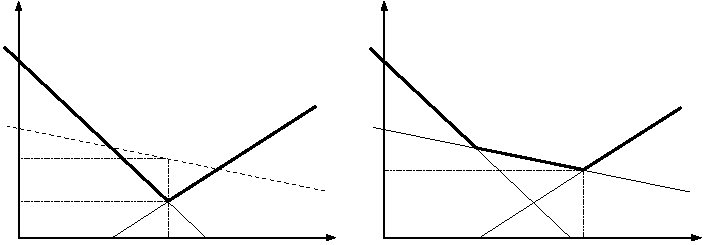
\includegraphics{part_1/chapter_2/figures/Figure4}};
		    \node (a) at (-4.5,0.2) {$a$};
			\node (ax=b) at (-3.6,-1.3) {$a^\top x =b$};
			\node (ax<b) at (-2.5, 0.8) {$a^\top x > b$};
			\node (ax>b) at (-2.3,-0.7) {$a^\top x < b$};
			\node (a1) at (1.5, -0.2) {$a_1$};
			\node (a2) at (2.8, 0.2) {$a_2$};
			\node (a3) at (1.8, 0.7) {$a_3$};
			\node (a4) at (2.9, -0.3) {$a_4$};
			\node (a5) at (2.2, -0.8) {$a_5$};
			\node[rotate = 90] (a1x=b1) at (0.1,0.2) {$a_1^\top x =b_1$};
			\node (a3x=b3) at (1.5,2.2) {$a_3^\top x =b_3$};
			\node (a2x=b2) at (4.5, 1) {$a_2^\top x =b_2$};
			\node (a4x=b4) at (4.4,-1.2) {$a_4^\top x =b_4$};
			\node (a5x=b5) at (1.3,-2) {$a_5^\top x =b_5$};
			\end{tikzpicture}
			\vspace{1pt}
		\caption{A hyperplane and its respective halfspaces (left) and the polyhedral set $\braces{x\in \reals^{2} : a_i^x \geq b_i, i =1,\dots, 5}$ (right).} \label{p1c2:fig:hyperplanes_and_polyhedral_set}		
	\end{figure}

You might find authors referring to bounded polyhedral sets as polytopes. However, this is not used consistently across references, sometimes with switched meanings (for example, using polytope to refer to a set defined as in Definition \ref{p1c2:def:polyhedral_sets} and using polyhedron to refer to a bounded version of $S$). In this text, we will only use the term polyhedral set to refer to sets defined as in Definition \ref{p1c2:def:polyhedral_sets} and use the term bounded whenever applicable.

Also, it may be useful to formally define some elements in polyhedral sets. For that, let us consider a hyperplane $H = \braces{x \in \reals^{n} : a^\top x = b}$, with $a \in \reals^n$ and $b \in \reals$. Now consider the set $F = H \cap S$. This set is known as a \emph{face} of a polyhedral set. If the face $F$ has dimension zero, then $F$ is called a vertex. Analogously, if $\dim(F)=1$, then $F$ is called an edge. Finally, if $\dim(F) = dim(S)-1$, then $F$ is called a facet. Notice that in $\reals^3$, facets and faces are the same, whenever the face is not an edge or a vertex. 


\subsection{Convexity of polyhedral sets}

As will see in more detail in Part 2 of this book, convexity plays a crucial role in optimisation, being the ``watershed'' between easy and hard optimisation problems. One of the main reasons why we can solve challenging linear programming problems is due to the inherent convexity of polyhedral sets.

Let us first define the notion of convexity for sets, which is stated in Definition \ref{p1c2:def:convex_set} 

\begin{definition}[Convex set]\label{p1c2:def:convex_set} 
	A set $S \subseteq \reals^n$ is convex if, for any $x_1,x_2 \in S$ and any $\lambda \in [0,1]$, we have that $\overline{x} = \lambda x_1 + (1-\lambda) x_2 \in S$.
\end{definition}

Definition \ref{p1c2:def:convex_set} leads to a simple geometrical intuition: for a set to be convex, the line segment connecting any two points within the set must lie within the set. This is illustrated in Figure \ref{p1c2:fig:convex_sets}.

\begin{figure}
	\begin{tikzpicture}
		\node (pic) at (0,0) {\includegraphics{part_1/chapter_2/figures/Figure5}};
		% Left pic line
		\node[circle, fill, minimum size=3pt, inner sep = 0pt] (x1) at (-4,-0.5) {};
		\node[above left] at (-4,-0.5) {$x_1$};
		\node[circle, fill, minimum size=3pt, inner sep = 0pt] (x2) at (-2.8,0.5) {};
		\node[above left] at (-2.8,0.5) {$x_2$};
		\draw[thick] (x1) -- (x2);
		% Center pic line
		\node[circle, fill, minimum size=3pt, inner sep = 0pt] (x1) at (-0.5,-0.5) {};
		\node[above left] at (-0.5,-0.5) {$x_1$};
		\node[circle, fill, minimum size=3pt, inner sep = 0pt] (x2) at (0.5,0.5) {};
		\node[above left] at (0.5,0.5) {$x_2$};
		\draw[thick] (x1) -- (x2);
		\node[circle, fill, minimum size=3pt, inner sep = 0pt] (x1) at (2.3, -0.3) {};
		\node[above] at (2.3, -0.3) {$x_1$};
		\node[circle, fill, minimum size=3pt, inner sep = 0pt] (x2) at (4,-0.3) {};
		\node[above left] at (4,-0.3) {$x_2$};
		\draw[thick] (x1) -- (x2);
	\end{tikzpicture}
	\caption{Two convex sets (left and middle) and one nonconvex set (right)} \label{p1c2:fig:convex_sets}
\end{figure}

Associated with the notion of convex sets are two important elements we will refer to later when we discuss linear problems that embed \emph{integrality requirements}. The first is the notion of a \emph{convex combination}, which is already contained in Definition \ref{p1c2:def:convex_set}, but can be generalised for an arbitrary number of points. The second consists of \emph{convex hulls}, which are sets formed by combining the convex combinations of all elements within a given set. As one might suspect, convex hulls are always convex sets, regardless of whether the original set from which the points are drawn from is convex or not. These are formalised in Definition \ref{p1c2:def:convex_combination_hull} and illustrated in Figure \ref{p1c2:fig:convex_hulls}.

\begin{definition}[Convex combinations and convex hulls] \label{p1c2:def:convex_combination_hull}
	Let $x_1, \dots, x_k \in \reals^n$ and $\lambda_1,\dots, \lambda_k \in \reals$ such that $\lambda_i \geq 0$ for $i = 1, \dots, k$ and $\sum_{i=1}^k \lambda_i = 1$. Then
	\begin{enumerate}
		\item $x = \sum_{i=1}^k \lambda_i x_i$ is a \emph{convex combination} of $\braces{x_i}_{i=1}^k \in \reals^n$;
		\item The \emph{convex hull} of $\braces{x_i}_{i=1}^k \in \reals^n$, denoted $\conv(x_1, \dots, x_k)$, is the set of all convex combinations of $\braces{x_i}_{i=1}^k \in \reals^n$.
	\end{enumerate}		
\end{definition}

\begin{figure}
	\begin{tikzpicture}
		\node (pic) at (0,0) {\includegraphics{part_1/chapter_2/figures/Figure6}};
		\node (x1l) at (-4.5,-0.7) {$x_1$};
		\node (x2l) at (-2.3, 0.7) {$x_2$};
		\node (x1c) at (-0.5, 1.1) {$x_1$};
		\node (x2c) at (0.8, -1) {$x_2$};
		\node (x3c) at (-1.5, -0.9) {$x_3$};
		\node (x1r) at (2.1, 1) {$x_1$};
		\node (x2r) at (4.4, 0.6) {$x_2$};
		\node (x3r) at (4.5, -0.9) {$x_3$};
		\node (x4r) at (1.9, -0.9) {$x_4$};
		\node (x5r) at (2.7, 0.4) {$x_5$};
		\node (x6r) at (3.8, -0.15) {$x_6$};
	\end{tikzpicture}
	\vspace{-6pt}
	\caption{The convex hull of two points is the line segment connecting them (left); The convex hull of three (centre) and six (right) points in $\reals^2$} \label{p1c2:fig:convex_hulls}
\end{figure}	

We are now ready to state the result that guarantees the convexity of polyhedral sets of the form
$$
	S = \braces{x \in \reals^n : Ax \le b}.
$$


\begin{theorem}[Convexity of polyhedral sets] \label{p1c2:thm:convexity}
	The following statements are true:
	\begin{enumerate}
		\item The intersection of convex sets is convex
		\item Every polyhedral set is a convex set
		\item A convex combination of a finite number of elements of a convex set also belongs to that set
		\item The convex hull of a finite number of elements is a convex set.			
	\end{enumerate}
\end{theorem}

\begin{proof}
	We provide the proof for each of the statements individually. 
	\begin{enumerate}
	 \item Let 	$S_i$, for $i \in I = \braces{1,\dots,n}$, be a collection of $n$ convex sets and suppose that $x, y \in \bigcap_{i \in I} S_i$. Let $\lambda \in [0,1]$. Since $S_i$ are convex and $x,y \in S_i$ for all $i \in I$, $\lambda x + (1-\lambda) y \in S_i$ for all $i \in I$ and, thus, $\lambda x + (1-\lambda) y \in \bigcap_{i \in I} S_i$.
	
	\item Let $a \in \reals^n$ and $b \in \reals$. Let $x,y \in \reals^n$, such that $a^\top x \geq b$ and $a^\top y \geq b$. Let $\lambda \in [0,1]$. Then $a^\top (\lambda x + (1-\lambda)y) \geq \lambda b + (1-\lambda)b = b$, showing that half-spaces are convex. The result follows from combining this with (1).    
	
	\item By induction. Let $S$ be a convex set and assume that the convex combination of $x_1, \dots, x_k \in S$ also belongs to $S$. Consider $k+1$ elements $x_1, \dots, x_{k+1} \in S$ and $\lambda_1, \dots, \lambda_{k+1}$ with $\lambda_i \in [0,1]$ for $i = 1,\dots, k+1$ and $\sum_{i=1}^{k+1}\lambda_i = 1$ and $\lambda_{k+1} \neq 1$ (without loss of generality). Then

	\begin{equation}
		\sum_{i=1}^{k+1}\lambda_i x_i = \lambda_{k+1}x_{k+1} + (1 - \lambda_{k+1}) \sum_{i=1}^k \frac{\lambda_i}{1 - \lambda_{k+1}}x_i. \label{p1c2:eq:induction}
	\end{equation}								

		Notice that $\sum_{i=1}^{k}\frac{\lambda_i}{1 - \lambda_{k+1}} = 1$. Thus, using the induction hypothesis, $\sum_{i=1}^{k}\frac{\lambda_i}{1 - \lambda_{k+1}}x_i \in S$. Considering that $S$ is convex and using \eqref{p1c2:eq:induction}, we conclude that $\sum_{i=1}^{k+1}\lambda_{k+1}x_{k+1} \in S$, completing the induction.
		
	\item Let $S = \conv(x_1, \dots, x_k)$. Let $y = \sum_{i=1}^k \alpha_i x_i$ and $z = \sum_{i=1}^k \beta_ix_i$ be such that $y,z \in S$, $\alpha_i,\beta_i \geq 0$, and $\sum_{i=1}^k \alpha_i = \sum_{i=1}^k \beta_i = 1$. Let $\lambda \in [0,1]$. Then
		%
		\begin{equation}
			\lambda y + (1- \lambda)z = \lambda\sum_{i=1}^k \alpha_i x_i + (1-\lambda)\sum_{i=1}^k \beta_i x_i = \sum_{i=1}^k (\lambda \alpha_i + (1-\lambda) \beta_i)x_i. 	
		\end{equation}
		%
		Since $\sum_{i=1}^k \lambda \alpha_i + (1-\lambda) \beta_i = 1$ and $\lambda \alpha_i + (1-\lambda) \beta_i \geq 0$ for $i=1,\dots,k$, $\lambda y + (1- \lambda)z$ is a convex combination of $x_1, \dots, x_k$ and, thus, $\lambda y + (1- \lambda)z \in S$, showing the convexity of $S$. \qedhere	
	\end{enumerate}	
\end{proof}

Figure \ref{p1c2:fig:convexity_theorem_examples} illustrates some of the statements represented in the proof. For example, the intersection of the convex sets is always a convex set. One should notice however that the same does not apply to the union of convex sets. Notice that statement 2 proves that polyhedral sets as defined according to Definition \ref{p1c2:def:polyhedral_sets} are convex. Finally the third figure on the right illustrates the convex hull of four points as a convex polyhedral set containing the lines connecting any two points within the set. 
 
\begin{figure}
	\begin{tikzpicture}
%			\draw[help lines] (-5,-1) grid (5,1);
		\node (pic) at (0,0) {\includegraphics{part_1/chapter_2/figures/Figure7}};
	\end{tikzpicture}
    \vspace{-6pt}
	\caption{Illustration of statement 1 (left), 2 (centre), and 3 and 4 (right)} \label{p1c2:fig:convexity_theorem_examples}
\end{figure}	

We will halt our discussion about convexity for now and return to it in deeper detail in Part 2. We finish by showing a simple yet very powerful result, which states that the presence of convexity is what allows us to conclude that a locally optimal solution returned by an optimisation algorithm applied to a linear programming problem is indeed optimal for the problem at hand. It so turns out that, in the context of linear programming, convexity is a given since linear functions are convex by definition and the feasibility set of linear programming is also convex (as we have just shown in \ref{p1c2:thm:convexity}).

\begin{theorem}[Global optimality for convex problems] \label{p1c2:thm:convexity_and_optimality}
 Let $f: \reals^n \to \reals$ be a convex function, that is, $f(\lambda x_1 + (1-\lambda)x_2) \le \lambda f(x_1) + (1-\lambda)f(x_2), \ \lambda \in [0,1]$, and let $S \subset \reals^n$ be a convex set. Let $x^*$ be an element of $S$. Suppose that $x^*$ is a local optimum for the problem of minimising $f(x)$ over $S$. That is, there exists some $\epsilon > 0$ such that $f(x^*) \leq f(x)$ for all $x \in S$ for which $\|x - x^*\| \leq \epsilon$. Then, $x^*$ is globally optimal, meaning that $f(x^*) \leq f(x)$ for all $x \in S$. 
\end{theorem}

\begin{proof}
	Suppose, in order to derive a contradiction that $f(x) < f(x^*)$ for some $x \in S$. Using Definition \ref{p1c2:def:convex_set}, we have that
	$$f(\lambda x + (1-\lambda) x^*) \le \lambda f(x) + (1-\lambda) f(x^*) < \lambda f(x^*) + (1-\lambda) f(x^*) = f(x^*), \ \forall \lambda \in [0,1].$$
	
	We see that the strict inequality $f(\lambda x + (1-\lambda) x^*) < f(x^*)$ holds for any point $\lambda x + (1-\lambda) x^*$, including those with $\| \lambda x + (1-\lambda) x^* - x^* \| \le \epsilon$. Our assumption thus contradicts the local optimality of $x^*$, and this proves that $f(x) \ge f(x^*)$ for all $x \in S$.
\end{proof}




\section{Extreme points, vertices, and basic feasible solutions}

Now we focus on the algebraic representation of the most relevant geometric elements in the optimisation of linear programming problems. As we have seen in the graphical example in the previous chapter, the optimum of linear programming problems is generally located at the vertices of the feasible set. Furthermore, such vertices are formed by the intersection of $n$ constraints (in a $n$-dimensional space, which comprises constraints that are active (or satisfied at the boundary of the half-space of said constraints).

First, let us formally define the notions of vertex and extreme point. Although in general these can refer to different objects, we will see that in the case of linear programming problems, if a point is a vertex, then it is an extreme point as well, the converse also being true.

\begin{definition}[Vertex] \label{p1c2:def:vertex}
	Let $P$ be a convex polyhedral set. The vector $x \in P$ is a vertex of $P$ if there exists some $c$ such that $c^\top x < c^\top y$ for all $y \in P$ with $y \neq x$.
\end{definition}

\begin{definition}[Extreme points]\label{p1c2:def:extreme_point}
	Let $P$ be a convex polyhedral set. The vector $x \in P$ is an extreme point of $P$ if there are no two vectors $y,z \in P$ (different than $x$) such that $x = \lambda y + (1 - \lambda)z$, for any $\lambda \in [0,1]$.
\end{definition}

Figure \ref{p1c2:fig:vertex_and_extreme_point} provides an illustration of the Definitions \ref{p1c2:def:vertex} and \ref{p1c2:def:extreme_point}. Notice that the definition of a vertex involves an additional hyperplane that, once placed on a vertex point, strictly contains the whole polyhedral set in one of the half-spaces it defines, except for the vertex itself. On the other hand, the definition of an extreme point only relies on convex combinations of elements in the set itself. 

\begin{figure}
	\begin{tikzpicture}
		\node (pic) at (0,0) {\includegraphics{part_1/chapter_2/figures/Figure8}};
		\node (Pl) at (-2.5, 0) {$P$};
		\node (Pr) at (3, 0) {$P$};
		\node (wl) at (-3, 0.9) {$w$};
		\node (xl) at (-2.3, -1.5) {$x$};
		\node (c1) at (-4, -1) {$c$};
		\node (c2) at (-0.9, -0.5) {$c$};
		\node[left] (cw) at (-2.3, 1.5) {$\braces{y : c^\top y = c^\top w}$};
		\node[right] (cx) at (-1.7, -1.4) {$\braces{y : c^\top y = c^\top x}$};
		\node (wr) at (2.1, 0.7) {$w$};
		\node (vr) at (2.4, 0.9) {$v$};
		\node (ur) at (1.8, 0.4) {$u$};
		\node (xr) at (3.1, -1.5) {$x$};
		\node (yr) at (3.4, -1.2) {$y$};
		\node (zr) at (2.8, -1.8) {$z$};
	\end{tikzpicture}
	\caption{Representation of a vertex (left) and a extreme point (right)} \label{p1c2:fig:vertex_and_extreme_point}
\end{figure}	

Definition \ref{p1c2:def:vertex} also hints an important consequence for linear programming problems. As we seen from Theorem \ref{p1c2:thm:convexity}, $P$ is convex, which guarantees that $P$ is contained in the half-space $c^\top y > c^\top x$. This  implies that $c^\top x \leq c^\top y, \forall y \in P$, which is precisely the condition that $x$ must satisfy to be the minimum for the problem $\mini_x\braces{c^\top x :x \in P}$.   

Now we focus on the description of active constraints from an algebraic standpoint. For that, let us first generalise our setting by considering all possible types of linear constraints. That is, let us consider the convex polyhedral set $P \subset \reals^n$, formed by the set of inequalities and equalities:
%
\begin{align*}
	& a_i^\top x \geq b, i \in M_1, \\ 
	& a_i^\top x \leq b, i \in M_2, \\
	& a_i^\top x = b, i \in M_3.
\end{align*}

\begin{definition}[Active (or binding) constraints] \label{p1c2:fig:active_constraint}
	If a vector $\overline{x}$ satisfies $a_i^\top \overline{x} = b_i$ for some $i \in M_1, M_2$, or $M_3$, we say that the corresponding constraints are active (or binding).
\end{definition}

Definition \ref{p1c2:fig:active_constraint} formalises the notion of active constraints. This is illustrated in Figure \ref{p1c2:fig:active_constraints}, where the polyhedral set $P = \braces{x \in \reals^3 : x_1 + x_2 + x_3 = 1, x_i \geq 0, i =1,2,3}$ is represented. Notice that, while points $A$, $B$, $C$ and $D$ have 3 active constraints, $E$ only has 2 active constraints ($x_2 = 0$ and $x_1 + x_2 + x_3 = 1$).

\begin{figure}[h]
	\begin{tikzpicture}
		\node (pic) at (0,0) {\includegraphics{part_1/chapter_2/figures/Figure9}};
		\node (x1) at (1.5, -2) {$x_1$};
		\node (x2) at (1.7, 0.4) {$x_2$};
		\node (x3) at (-2.1, 2) {$x_3$};
		\node (P) at (0, -0.5) {$P$};
		\node[left] (A) at (-1.1, 1.3) {$A$};
		\node[left] (B) at (-1.8, -1) {$B$};
		\node[right] (C) at (-0.5, -1.9) {$C$};
		\node[above] (D) at (0.9, -0.1) {$D$};
		\node[right] (E) at (-1.6, -0.2) {$E$};
	\end{tikzpicture}
	\caption{Representation of $P$ in $\reals^3$.} \label{p1c2:fig:active_constraints}
\end{figure}	

Theorem \ref{p1c2:thm:active_const} sows a thread between having a collection of active constraints forming a vertex and being able to describe it as a basis of a subspace that is formed by the vectors $a_i$ that form these constraints. This link is what will allow us to characterise vertices by their forming active constraints.

\begin{theorem}[Properties of active constraints]\label{p1c2:thm:active_const}
	Let $\overline{x} \in \reals^n$ and $I = \braces{ i \in M_1 \cup M_2 \cup M_3 : a_i^\top \overline{x} = b_i}$. Then, the following are equivalent:
	\begin{enumerate}
		\item There exists $n$ vectors in $\braces{a_i}_{i \in I}$ that are linearly independent.  
		\item The $\spans(\braces{a_i}_{i \in I})$ spans $\reals^n$. That is, every $x \in \reals^n$ can be expressed as a linear combination of $\braces{a_i}_{i \in I}$.
		\item The system of equations $\braces{a_i ^\top x = b_i}_{i \in I}$ has a unique solution.
	\end{enumerate}
\end{theorem}

\begin{proof}
	Suppose that $\braces{a_i}_{i \in I}$ spans $\reals^n$, implying that the $\spans(\braces{a_i}_{i \in I})$ has dimension $n$. By Theorem \ref{p1c2:thm:LI_and_bases} (part 1), $n$ of these vectors form a basis for $\reals^n$ and are, thus, linearly independent. Moreover, they must span $\reals^n$ and therefore every $x \in \reals^n$ can be expressed as a combination of $\braces{a_i}_{i \in I}$. This connects (1) and (2).
	
	Assume that the system of equations $\braces{a_i ^\top x = b_i}_{i \in I}$ has multiple solutions, say $x_1$ and $x_2$. Then, the nonzero vector $d = x_1 - x_2$ satisfies $a_i^\top d = 0$ for all $i \in I$. As $d$ is orthogonal to every $a_i$, $i \in I$, $d$ cannot be expressed as a combination of $\braces{a_i}_{i \in I}$ and, thus, $\braces{a_i}_{i \in I}$ do not span $\reals^n$.
	
	Conversely, if $\braces{a_i}_{i \in I}$ do not span $\reals^n$, choose $d \in \reals^n$ that is orthogonal to $\spans(\braces{a_i}_{i \in I})$. If $x$ satisfies $\braces{a_i ^\top x = b_i}_{i \in I}$, so does $\braces{a_i ^\top (x + d) = b_i}_{i \in I}$, thus yielding multiple solutions. This connects (2) and (3). \qedhere
\end{proof}

Notice that Theorem \ref{p1c2:thm:active_const} implies that there are (at least) \emph{$n$ active constraints ($a_i$)} that are \emph{linearly independent} at $\overline{x}$. This is the reason why we will refer to $\overline{x}$, and any vertex-forming solution, as a \emph{basic solution}, of which we will be interested in those that are feasible, i.e., that satisfy all constraints $i \in M_1 \cup M_2 \cup M_3$. Definition \ref{p1c2:def:basic_feasible_solution} provides a formal definition of these concepts.

\begin{definition}[Basic feasible solution (BFS)] \label{p1c2:def:basic_feasible_solution}
	Consider a convex polyhedral set $P \subset \reals^n$ defined by linear equality and inequality constraints, and let $\overline{x} \in \reals^n$.
	\begin{enumerate}
		\item $\overline{x}$ is a \emph{basic solution} if 
		\begin{enumerate}
			\item All equality constraints are active,
			\item Out of the constraints active at $\overline{x}$, $n$ of them are linearly independent, and
			\item $\overline{x}$ is the unique solution of the linear system formed by $n$ linearly-independent active constraints.
		\end{enumerate}
		\item if $\overline{x}$  is a basic solution satisfying all constraints, we say $\overline{x}$ is a basic feasible solution. 
	\end{enumerate}
\end{definition}

Figure \ref{p1c2:fig:BFS} provides an illustration of the notion of basic solutions, and show how only a subset of the basic solutions are feasible. As one might infer, these will be the points of interest in out future developments, as these are the candidates for optimal solution.

\begin{figure}[h]
	\begin{tikzpicture}
		\node (pic) at (0,0) {\includegraphics{part_1/chapter_2/figures/Figure10}};
		\node[above] (A) at (-0.7, 1) {$A$};
		\node[left] (B) at (-0.9, 0.2) {$B$};
		\node[right] (C) at (-0.4, 0.7) {$C$};
		\node[below] (D) at (1.6, -1.2) {$D$};
		\node[below] (E) at (-0.5, -1) {$E$};
		\node[above] (F) at (-1.8, -0.8) {$F$};
		\node (P) at (-0.3, -0.3) {$P$};
	\end{tikzpicture}
	\caption{Points $A$ to $F$ are basic solutions; $B$,$C$,$D$, and $E$ are BFS.} \label{p1c2:fig:BFS}
\end{figure}		

We finalise stating the main result of this chapter, which formally confirms the intuition we have developed so far. That is, for convex polyhedral sets, the notion of vertices and extreme points coincide, and these points can be represented as basic feasible solutions. This is precisely the link that allows for considering the feasible region of linear programming problems under a purely algebraic characterisation of the candidates for optimal solutions, those described uniquely by a subset of constraints of the problem that is assumed to be active.

\begin{theorem}[BFS, extreme points and vertices]\label{p1c2:thm:BFS_vertex_extreme_point}
	Let $P \subset \reals^n$ be a convex polyhedral set and let $\overline{x} \in P$. Then, the following are equivalent
	$$	\overline{x} \text{ is a vertex} \iff \overline{x} \text{ is an extreme point} \iff \overline{x} \text{ is a BFS}.	
	$$
\end{theorem}


\begin{proof}
	Let $P =\{ x \in \reals^n : a_i^\top x \geq b_i, i \in M_1, a_i^\top x = b_i, i \in M_2\}$, and $I = \braces{i \in M_1 \cup M_2 \mid a_i^\top x = b_i}$.
	
	\begin{enumerate}
		\item (Vertex $\Rightarrow$ Extreme point) Suppose $\overline{x}$ is a vertex. Then, there exists some $c \in \reals^n$ such that $c^\top\overline{x} < c^\top x$, for every $x \in P$ with $x \neq \overline{x}$ (cf. Definition \ref{p1c2:def:vertex}). Take $y,z \in P$ with $y,z \neq \overline{x}$. Thus $c^\top\overline{x} < c^\top y$ and $c^\top\overline{x} < c^\top z$. For $\lambda \in [0,1]$, $c^\top \overline{x} < c^\top(\lambda y + (1-\lambda)z)$ implying that $\overline{x} \neq \lambda y + (1-\lambda)z$, and is thus an extreme point (cf. Definition \ref{p1c2:def:extreme_point}).
		
		\item (Extreme point $\Rightarrow$ BFS) We will prove the contrapositive instead\footnote{Consider two propositions $A$ and $B$. Then, we have that $A \Rightarrow B \equiv \neg B \Rightarrow \neg A$. The latter is known as the \emph{contrapositive} of the former.}. Suppose $\overline{x} \in P$ is not a BFS. Then, there are no $n$ linearly independent vectors within $\braces{a_i}_{i \in I}$. Thus the vectors  $\braces{a_i}_{i \in I}$ lie in a proper subspace of $\reals^n$. Let the nonzero vector $d \in \reals^n$ be such that $a_i^\top d = 0$, for all $i \in I$.
			
			Let $\epsilon > 0$, $y = \overline{x} + \epsilon d$, and $z = \overline{x} - \epsilon d$. Notice that $a_i^\top y = a_i^\top z = b_i$, for all $i \in I$. Moreover, for $i \neq I$, $a_i^\top x > b_i$ and, provided that $\epsilon$ is sufficiently small (such that $\epsilon|a_i^\top d| < a_i ^\top \overline{x} - b_i $), we have that $a_i ^\top x \geq b_i$ for all $i \in I$. Thus $y \in P$, and by a similar argument, $z \in P$. Now, by noticing that $\overline{x} = \frac{1}{2}y + \frac{1}{2}z$, we see that $\overline{x}$ is not an extreme point. 			 
		\item (BFS $\Rightarrow$ Vertex) Let $\overline{x}$ be a BFS. Define $c = \sum_{i \in I} a_i$. Then
			\begin{equation*}
				c^\top \overline{x} = \linebreak \sum_{i \in I} a_i^\top \overline{x} = \sum_{i \in I} b_i.	 			 	
	 		\end{equation*}
			Also, for any $x \in P$, we have that 
			\begin{equation*}
				c^\top x = \sum_{i \in I} a_i^\top x \geq \sum_{i \in I} b_i, 	 	
	 		\end{equation*}
	 		since $a_i^\top x \geq b_i$ for $i \in M_1 \cup M_2$. Thus, for any $x \in P$, $c^\top \overline{x} \leq c^\top x$, making $\overline{x}$ a vertex (cf. Definition \ref{p1c2:def:vertex}). \qedhere
	\end{enumerate} 	
\end{proof}

Some interesting insights emerge from the proof of Theorem \ref{p1c2:thm:BFS_vertex_extreme_point}, upon which we will build our next developments. Once the relationship between being a vertex/extreme point and a BFS is made, it means that $\overline{x}$ can be recovered as the unique solution of a system of linear equations, these equations being the active constraints at that vertex. This means that the list of all optimal solution candidate points can be obtained by simply looking at all possible combinations of $n$ active constraints, discarding those that are infeasible. This means that the number of candidates for optimal solution is \emph{finite} and can be bounded by $\binom{m}{n}$, where $m=| M_1 \cup M_2 |$. 

\vfill
\pagebreak
\section{Exercises}

\subsection*{Exercise 2.1: Polyhedral sets \cite{bertsimas1997introduction}}
Which of the following sets are polyhedral sets?

\begin{itemize}
	\item[a)] $\{(x,y)\in\mathbb{R}^2~|~ x \cos \theta + y\sin\theta \leq 1,\theta\in[0,\pi/2],x\geq0,y\geq0\}$
	\item[b)] $\{x\in\mathbb{R}~|~ x^2-8x+15\leq 0\}$
	\item[c)] The empty set ($\emptyset$).
\end{itemize}

\subsection*{Exercise 2.2: Convexity of polyhedral sets}
Prove the following theorem.

\begin{theorem*}[Convexity of polyhedral sets] 
	%	\vspace{-3pt}
	\emph{The following convexity properties about convex sets can be said:}
	\begin{enumerate}
		\item The intersection of convex sets is convex
		\item Every polyhedral set is a convex set
		\item A convex combination of a finite number of elements of a convex set also belongs to that set
		\item The convex hull of a finite number of elements is a convex set.			
	\end{enumerate}
\end{theorem*}

Note: the proof of the theorem is proved in the notes. Use this as an opportunity to revisit the proof carefully, and try to take as many steps without consulting the text as you can. This is a great exercise to help you internalise the proof and its importance in the context of this book. I strongly advise against blindly memorising it, as I suspect you will never (in my courses, at least) be requested to recite the proof literally.


\subsection*{Exercise 2.3: Inverses, linear independence, and solving $Ax = b$} 
Prove the following theorem.

\begin{theorem*}[Inverses, linear independence, and solving $Ax = b$]
	Let $A$ be a $m \times m$ matrix. Then, the following statements are equivalent:
	\begin{enumerate}
		\item $A$ is invertible
		\item $A^\top$ is invertible
		\item The determinant of $A$ is nonzero
		\item The rows of $A$ are linearly independent
		\item The columns of $A$ are linearly independent
		\item For every $b \in \reals^m$, the linear system $Ax = b$ has a unique solution
		\item There exists some $b \in \reals^m$ such that $Ax = b$ has a unique solution.	
	\end{enumerate}	
\end{theorem*}


\subsection*{Exercise 2.4: Linear independence}
\begin{itemize}
	\item[a)] According to Theorem \ref{p1c2:thm:fundamental_linear_algebra}, if the columns (or rows) of the $m \times m$ matrix $A$ are linearly independent, the system $Ax=b$ has a unique solution for every vector $b$. Explain the significance of this result in the context of linear optimization.
	\item[b)] If the columns of $A$ are not linearly independent, the system $Ax = b$ has either no solution or infinitely many solutions. Using the notions of \emph{span} and \emph{proper subspace}, explain why this is the case. 
	\item[c)] Solve the following systems of equations. Based on your findings, which systems have an invertible coefficient matrix?
	\begin{itemize}
		\item[] \begin{align*}
			2x_1 + 3x_2 + x_3 &= 12\\
			x_1 + 2x_2 + 3x_3 &= 12\\
			3x_1 + x_2 + 2x_3 &= 12
		\end{align*}
		\item[] \begin{align*}
			x_1 + 2x_2 + 4x_3 &= 6\\
			2x_1 + x_2 + 5x_3 &= 6\\
			x_1 + 3x_2 + 5x_3 &= 6
		\end{align*}
		\item[] \begin{align*}
			x_1 + 2x_2 + 4x_3 &= 5\\
			2x_1 + x_2 + 5x_3 &= 4\\
			x_1 + 3x_2 + 5x_3 &= 7
		\end{align*}
	\end{itemize}
\end{itemize}


\subsection*{Exercise 2.5: Properties of active constraints}
Let us consider the convex polyhedral set $P \subset \reals^n$, formed by the set of equalities and inequalities:
%
\begin{align*}
	a_i^\top x \geq b, i \in M_1, \\
	a_i^\top x \leq b, i \in M_2, \\
	a_i^\top x = b, i \in M_3.
\end{align*}
%

Prove the following result.

\begin{theorem*}[Properties of active constraints]
	Let $\overline{x} \in \reals^n$ and $I = \braces{ i \in M_1 \cup M_2 \cup M_3 \mid a_i^\top \overline{x} = b_i}$. Then, the following are equivalent:
	\begin{enumerate}
		\item There exists $n$ vectors in $\braces{a_i}_{i \in I}$ that are linearly independent.  
		\item The $\spans(\braces{a_i}_{i \in I})$ spans $\reals^n$. That is, every $x \in \reals^n$ can be expressed as a combination of $\braces{a_i}_{i \in I}$.
		\item The system of equations $\braces{a_i ^\top x = b_i}_{i \in I}$ has a unique solution.
	\end{enumerate}
\end{theorem*}

Note: see Exercise 2.2.

\subsection*{Exercise 2.6: Vertex, extreme points, and BFSs}
Prove the following result.

\begin{theorem*}[BFS, extreme points and vertices]
	Let $P \subset \reals^n$ be a convex polyhedral set and let $\overline{x} \in P$. Then, the following are equivalent
	\begin{enumerate}
		\item $\overline{x}$ is a vertex;
		\item $\overline{x}$ is a extreme point;
		\item $\overline{x}$ is a BFS;	
	\end{enumerate}
\end{theorem*}

Note: see Exercise 2.2.

\subsection*{Exercise 2.7: Binding constraints} 
Given the linear program defined by the system of inequalities below,
%
\begin{flalign*}
	\maxi & 2x_1 + x_2 && \\
	\st   & 2x_1 + 2x_2 \leq 9 && \\
		  & 2x_1 - x_2 \leq 3 && \\
		  & x_1 - x_2 \leq 1 && \\
		  & x_1 \leq 2.5 && \\
		  & x_2 \leq 4 && \\
		  & x_1, x_2 \geq 0.
\end{flalign*}
%
Assess the following points relative to the polyhedron defined in $\reals^2$ by this system and classify them as in $(i)$ belonging to which active constraint(s), $(ii)$ being a non-feasible/basic/basic feasible solution, and $(iii)$ being an extreme point, vertex, or outside the polyhedron. Use Theorem \ref{p1c2:thm:active_const} and Theorem \ref{p1c2:thm:BFS_vertex_extreme_point} to check if your classification is correct.

\begin{itemize}
	\item[a)] $(1.5,0)$
	\item[b)] $(1,0)$
	\item[c)] $(2,1)$
	\item[d)] $(1.5,3)$
\end{itemize}

 

